\documentclass[12pt,a4paper,oneside]{article}
\usepackage{graphicx}
\usepackage{titlepic}
\usepackage[utf8]{inputenc}
\usepackage[left=1.1in,right=1.1in, top=1in, bottom= 1in]{geometry}
\usepackage{amsfonts}
\usepackage{amssymb}
\usepackage{amsmath}
\usepackage{fancyhdr}
\usepackage{hyperref}
\usepackage{etoolbox}
\usepackage[nottoc]{tocbibind}
\usepackage{appendix}
\usepackage{multicol}
\usepackage{leftidx}
\graphicspath{{figures/}}
\usepackage{ragged2e}
\usepackage{mathtools}
\usepackage{units}
\usepackage{float}
\usepackage{subcaption}
\usepackage{commath}

\usepackage{amsthm}

\theoremstyle{definition}
\newtheorem{definition}{Definition}[section]

\newtheorem{theorem}{Theorem}

\usepackage[none]{hyphenat} % Avoids to go out of margin

\usepackage{subfiles}

% --------------------------------------------- %

\title{Simulazione Crescita Cristallina}	% Title
\author{Francesco Di Monaco (1988475)  \\ Vincenzo Malanga (2024764)} % Authors separated by \\
\date{30/05/2024}	% Date

% Font size of figure smaller than normal size:
\usepackage{caption}
\captionsetup[figure]{font=small}
%\captionsetup[table]{font=small}

%\usepackage{setspace} % double spacing
\linespread{1.2}

\makeatletter
\let\thetitle\@title
\let\theauthor\@author
\let\thedate\@date
\makeatother

\begin{document}

\begin{titlepage}
	\centering
    \vspace*{0.5 cm}
    
\includegraphics[scale = 0.75]{figures/SapienzaLogo.pdf}\\[1.0 cm]	% University Logo

    \vspace*{-0.4cm}
    \textsc{\large Dipartimento di Informatica}\\[2.0 cm]	% Department Name
    \vspace*{1cm}

    { \fontsize{20.74pt}{18.5pt}\selectfont\bfseries \thetitle \par } % Title

    \vspace*{0.25cm}
    \textsc{\Large Programmazione di Sistemi Embedded e Multicore}\\[0.5 cm] % Course Name

    \vspace*{2.6cm}
	\begin{minipage}{0.4\textwidth} % 0.4
		\begin{flushleft} \large
			\textbf{Professore:}\\
			Salvatore Pontarelli\\
		\end{flushleft}
	\end{minipage}~
	\begin{minipage}{0.5\textwidth} %0.4
		\begin{flushright} \large
		\begin{minipage}{1\textwidth}
		\begin{flushleft} \large
			\textbf{Studenti:} \\
			\theauthor
        \end{flushleft}
        \end{minipage}
		\end{flushright}
	\end{minipage}\\[3.85 cm]

    \vspace{2cm}
    \rule{\linewidth}{0.2 mm} \\[0.3 cm]
    \vspace*{-0.2cm}
    Academic Year 2023/2024
\end{titlepage}
\newpage
\tableofcontents
\newpage

\section{Descrizione del progetto}
Diffusion-limited aggregation (DLA) è un processo di formazione di cristalli nel quale le particelle si muovono in uno spazio 2D con moto browniano (cioè in modo casuale) e si combinano tra loro quando si toccano. DLA può essere simulato utilizzando una griglia 2D in cui ogni cella può essere occupata da uno o più particelle in movimento. 
Una particella diventa parte di un cristallo (e si ferma) quando si trova in prossimità di un cristallo già formato. I parametri di base della simulazione sono la dimensione della griglia 2D, il numero iniziale di particelle, il numero di iterazioni e il "seme" cristallino iniziale.
Per la nostra simulazione abbiamo deciso di utilizzare i framework OpenMP e CUDA.

\section{Il nostro approccio}
L'obiettivo che ci siamo preposti consiste nel permettere alle particelle di muoversi liberamente in qualsiasi punto dello spazio, indipendentemente dalla griglia menzionata nella consegna. Per questo motivo, nella nostra architettura, le particelle occupano una zona di memoria separata da quella della griglia. In quest'ultima, infatti, sono memorizzati solo i puntatori alle particelle. \\ Ci teniamo a sottolineare che la griglia è utilizzata esclusivamente come supporto per l'algoritmo e non è necessaria per l'esistenza delle particelle stesse.
Per limitare notevolmente il numero di controlli necessari, abbiamo adottato approcci che includono memoization, caching e sfruttamento della località delle particelle. \\
Tutte le implementazioni utilizzano il 100\% delle risorse hardware.

 
\newpage
\section{Architettura}
Il nostro algoritmo è implementato tramite una matrice, le cui celle contengono una linked-list ciascuna.
Così facendo evitiamo la pre-allocazione preventiva di spazio per ogni cella, impiegando invece gli struct delle particelle come nodi delle linked-list. Ad ogni particella nello spazio corrisponde una cella della griglia, a seconda delle coordinate. La griglia viene popolata e svuotata a ogni iterazione.
Questa architettura ci consente di sfruttare la località delle particelle ed evitare controlli superflui.
La grandezza della matrice varia a seconda del parametro "Cell size", che è la misura del lato delle celle.

\begin{figure}[H]
    \centering
    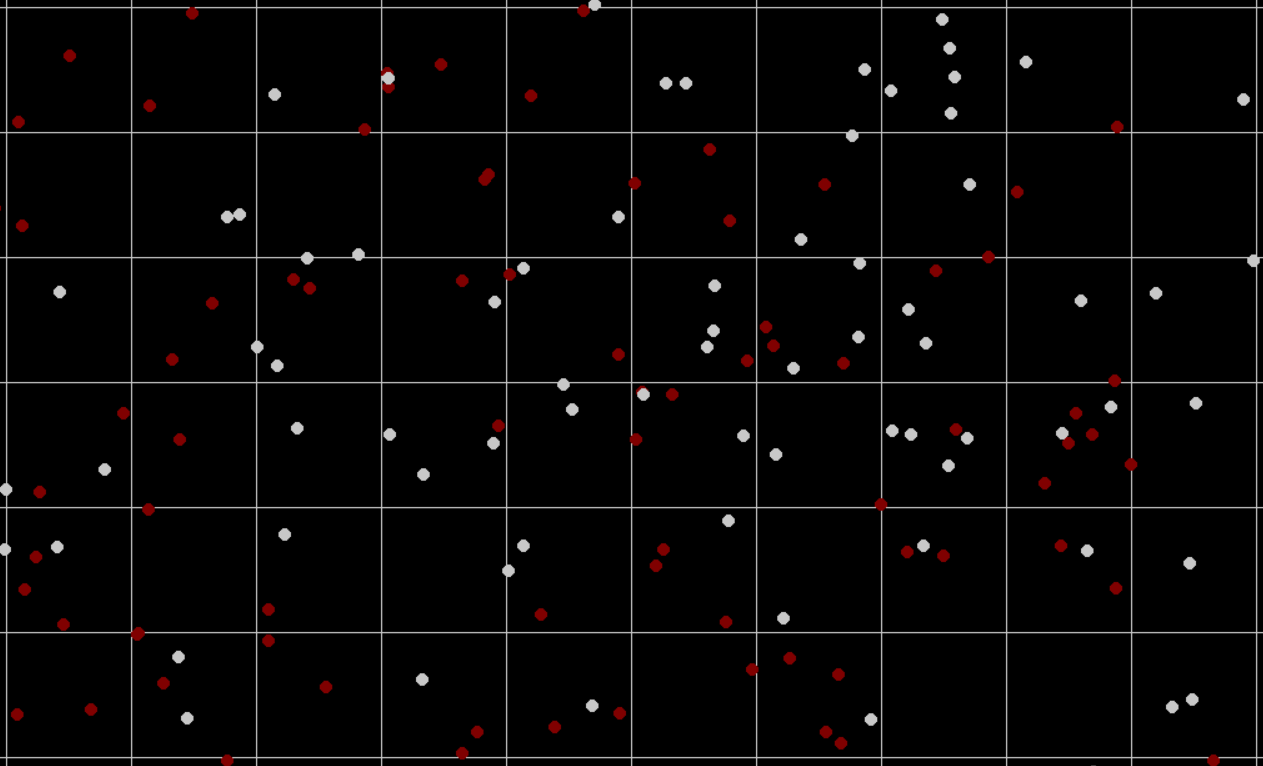
\includegraphics[width=1\linewidth]{griglia.png}
\end{figure}

\newpage

\section{Algoritmo}
Il nostro algoritmo prevede i seguenti passaggi:
\begin{enumerate}
    \item Popolare le celle della matrice con linked-list vuote.
    \item Popolare le linked-list con le particelle.
    \item Ordinare le linked-list.
    \item Verificare eventuali collisioni.
    \item Muovere le particelle.
    \item Ricominciare dal punto 1.
\end{enumerate}

\subsection{Popolare le celle della matrice con linked-list vuote}
In questa fase inizializziamo o resettiamo le teste delle linked-list, preparando così la matrice per il passaggio successivo: l'inserimento delle particelle. L'utilizzo delle linked-list è una scelta obbligata. Se avessimo optato per array di dimensione fissa, avremmo dovuto allocare molta memoria e sprecarne altrettanta. Un'alternativa sarebbe stata l'uso di ArrayList in ogni cella, ma questo avrebbe comunque comportato sprechi di memoria e difficoltà nell'implementare una struttura come l'ArrayList in CUDA. 

\subsection{Popolare le linked-list con le particelle}
Iteriamo sull’array delle particelle e per ognuna di esse inseriamo il puntatore nella cella corrispondente alle sue coordinate.
Questo passaggio richiede l'uso di lock o meccanismi di sincronizzazione per consentire l'inserimento nelle liste, garantendo così la thread-safety. In questa fase dell'algoritmo, l'implementazione può variare leggermente a seconda del framework utilizzato. \\ Ad esempio, in CUDA abbiamo incontrato difficoltà nell'implementazione di sezioni critiche con i lock, rendendo necessario l'utilizzo del check-and-set. In OpenMP, invece, l'implementazione è stata possibile solamente mediante l'utilizzo di lock mutex. 

\subsection{Ordinare le linked-list}
Ogni linked-list viene ordinata mediante un algoritmo di ordinamento. Questo passaggio è essenziale per rendere lineare la complessità del passaggio successivo. \\ Per comprendere meglio l'importanza di questa operazione, consideriamo il caso in cui non venisse eseguita: il passaggio successivo richiede la verifica delle collisioni tra coppie di celle. Se le particelle all'interno di queste celle non fossero ordinate, saremmo comunque costretti a utilizzare un algoritmo che renda questi controlli più efficienti, probabilmente attraverso processi simili all'ordinamento.
Ordinare le celle in anticipo ci permette di eseguire questi processi una sola volta per ogni cella, agendo come una sorta di memoizzazione.

 


\subsection{Verificare eventuali collisioni}
Iteriamo sulle celle della matrice e, per ciascuna di esse, controlliamo le collisioni con le particelle presenti nelle celle adiacenti. L'algoritmo sviluppato per la verifica delle collisioni prende in input due celle alla volta, quindi iteriamo sulla matrice e per ogni cella eseguiamo l’algoritmo n volte (sulle celle circostanti), dove n dipende dal tipo di cella*. Grazie al fatto che le linked-list presenti nelle celle sono ordinate, l’algoritmo può operare con complessità lineare, sfruttando la pseudo-memoizzazione del passaggio precedente.

\begin{figure}[H]
    \centering
    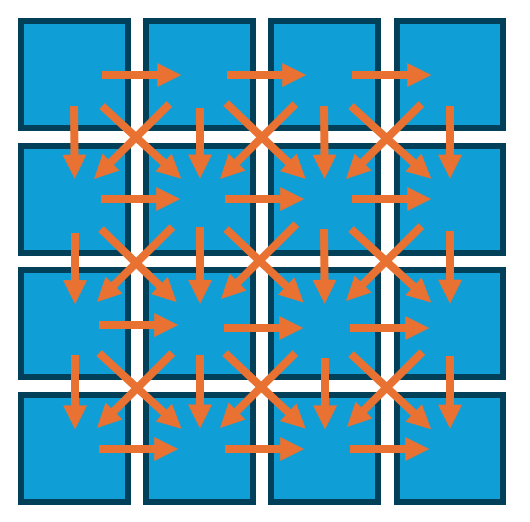
\includegraphics[width=0.8\linewidth]{patterns.png}
    \caption{Cell checking patterns}
    \label{fig:enter-label}
\end{figure}

\begin{quote}
 * Per evitare controlli ridondanti, abbiamo sviluppato dei pattern che, a seconda del tipo di cella, determinano quali celle adiacenti devono essere controllate, evitando di verificare tutte e nove le celle circostanti.
\end{quote}
 

\subsection{Muovere le particelle}
Iteriamo sull’array delle particelle ed in ogni struct cambiamo le coordinate di 1 pixel. La direzione è data da un random number generator.


\section{Problemi e migliorie}
Riteniamo che l'elemento meno efficiente del nostro algoritmo sia la necessità di svuotare e riempire nuovamente le liste collegate a ogni iterazione.
Una possibile soluzione sarebbe evitare di resettare le linked list e spostare soltanto le particelle che hanno effettivamente cambiato cella.

\newpage

\section{Performance}
Di seguito riportiamo le misuraizoni delle performance, con la dimensione delle celle e numero di particelle come parametri. Con alcune combinazioni di parametri si può notare come la versione single thread sia superiore alle versioni parallele. Attribuiamo questo fatto all'overhead causato dalla gestione dei thread, in combinazione con un numero ridotto di particelle.
\begin{figure}[H]
    \centering
    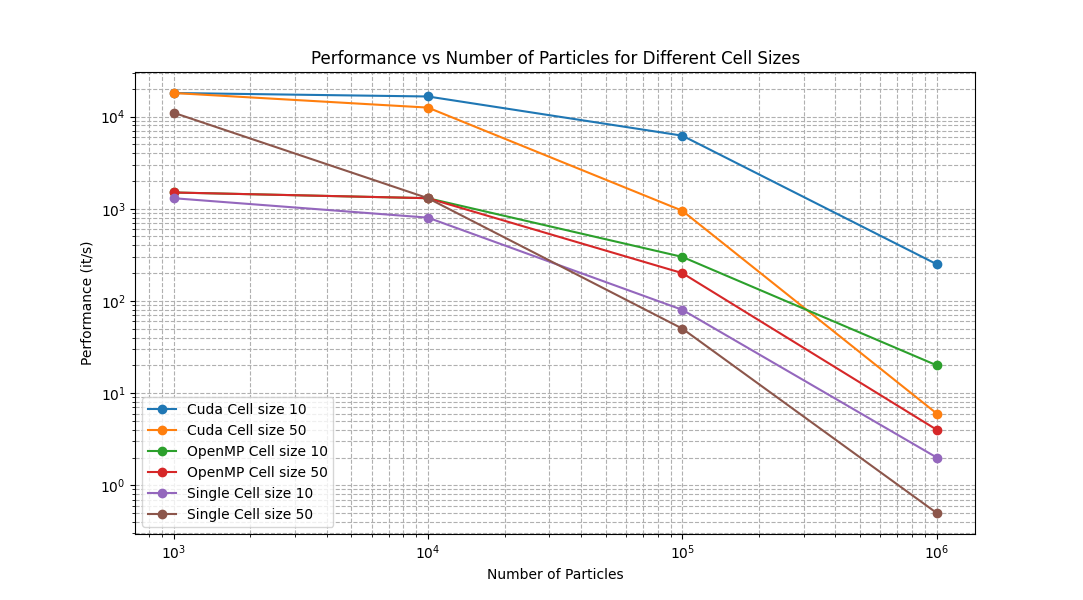
\includegraphics[width=1\linewidth]{Figure_1.png}
    \label{fig:enter-label}
\end{figure}

\begin{table}[H]
    \centering
    \begin{tabular}{cccc}
        \hline
        Particles & OpenMP (Cell Size 10) & CUDA (Cell Size 10) \\
        \hline
        1,000 & 13.3\% & 92.8\% \\
        10,000 & 38.5\% & 95.2\% \\
        100,000 & 73.3\% & 98.7\% \\
        1,000,000 & 90.0\% & 99.2\% \\
        \hline
    \end{tabular}
    \caption{Percentage improvement for cell size 10}
    \label{tab:percentage_improvement_cell_size_10}
\end{table}
\begin{table}[H]
    \centering
    \begin{tabular}{cccc}
        \hline
        Particles & OpenMP (Cell Size 50) & CUDA (Cell Size 50) \\
        \hline
        1,000 & \leq 0.0\% & 38.9\% \\
        10,000 & 0.0\% & 89.6\% \\
        100,000 & 75.0\% & 94.7\% \\
        1,000,000 & 87.5\% & 91.7\% \\
        \hline
    \end{tabular}
    \caption{Percentage improvement for cell size 50}
    \label{tab:percentage_improvement_cell_size_50}
\end{table}




\newpage
\clearpage
\bibliographystyle{unsrt}

\end{document}
